\documentclass{article}

% NeurIPS workshop style: drop neurips_2026.sty into this directory and
% uncomment before submission (use the target workshop's variant).
% \usepackage[final]{neurips_2026}

\usepackage[utf8]{inputenc}
\usepackage[T1]{fontenc}
\usepackage{hyperref}
\usepackage{url}
\usepackage{booktabs}
\usepackage{amsfonts,amsmath}
\usepackage{graphicx}
\usepackage{xcolor}
\usepackage[numbers]{natbib}
\newcommand{\todo}[1]{\textcolor{red}{[TODO: #1]}}
\newcommand{\jph}[1]{\textcolor{blue}{#1}} % judge-dependent placeholder

\title{Learning to Withdraw: Reflexive Environments as a Benchmark\\
for Long-Horizon Agent Memory}

\author{%
  Ariel Agor\\
  Independent Researcher\\
  \texttt{ariel@agor.me}\\
}

\begin{document}
\maketitle

\begin{abstract}
Benchmarks for LLM agents almost universally hold the environment's other actors fixed with respect to the agent's strategy. Real deployment settings are \emph{reflexive}: markets, negotiations, and multi-agent ecosystems adapt to the agent's observable behavior, so the agent's own participation shifts the process it is trying to predict. We introduce a deterministic, seeded commodity-market benchmark in which rule-based adversaries profile the focal agent's order flow and, once its behavior becomes predictable, exploit it through front-running and targeted spread-widening. We evaluate three memory architectures over 1{,}500--10{,}000-turn campaigns: a stateless baseline, a conventional episodic-summary-plus-retrieval memory, and a recursive \emph{self-model} architecture that maintains a token-capped, continuously rewritten identity file through a meta-cognitive audit loop. We find that reflexivity punishes engagement: the stateless agent, unable to represent that its own patterns are being exploited, keeps trading and is driven to ruin (mean campaign score $-1686$, exploited on 82\% of turns), while both memory architectures survive primarily by \emph{learning to withdraw} from the market. The self-model architecture withdraws reliably across all seeds and with explicit reflexive reasoning; the retrieval baseline withdraws erratically and on one seed re-engages catastrophically. We introduce a \emph{self-attribution} metric---whether the agent attributes environmental shifts to its own footprint rather than to exogenous shocks---scored blind by cross-family judges, and use it to test whether withdrawal is driven by correct reflexive reasoning \jph{(result pending)}. We report the emergent-withdrawal finding, its dependence on the environment's mean-reverting structure, and the higher compute cost and long-horizon brittleness of the self-model loop, as an honest characterization of what current agent memory does under reflexivity rather than a claim of architectural superiority. All hypotheses, metrics, and exclusion rules were pre-registered in version control before any run.
\end{abstract}

\section{Introduction}

The dominant evaluation paradigm for LLM agents assumes a fixed world. Benchmarks such as ALFWorld~\citep{shridhar2021alfworld}, WebArena~\citep{zhou2024webarena}, GAIA~\citep{mialon2023gaia}, $\tau$-bench~\citep{yao2024taubench}, and long-horizon suites like Vending-Bench~\citep{backlund2025vendingbench} and UltraHorizon~\citep{luo2025ultrahorizon} vary tasks, horizons, and noise, but the behavior-generating process of every other actor is stationary with respect to the focal agent's strategy. Soros's theory of reflexivity~\citep{soros1987alchemy,soros2013fallibility} names what this omits: in social systems, participants' models of the world alter the world, which alters the models. The phenomenon has a rigorous formulation in performative prediction~\citep{perdomo2020performative} and performative reinforcement learning~\citep{mandal2023performativerl}, where the deployed policy shifts the distribution it is evaluated on. No LLM-agent memory benchmark instantiates it: memory systems are tested on how much they can recall, not on whether they can recognize their own footprint in a world that is reacting to them.

This gap matters because the most consequential deployment environments---markets, negotiation, security, platform ecosystems---are the reflexive ones. An agent whose memory cannot distinguish ``the market changed'' from ``the market changed \emph{because of me}'' will misattribute self-induced adversarial adaptation to exogenous noise and keep feeding the exploit.

We set out to test a natural hypothesis: that a recursive self-model memory---an agent that maintains and continuously rewrites an explicit representation of its own strategy, biases, and situation---would confer an advantage in reflexive environments over conventional memory. What we found is more interesting than the hypothesis, and we report it as such. Reflexivity does not primarily reward better trading; it \emph{punishes engagement}. The winning behavior our agents discover is to stop acting once acting becomes dangerous. Memory is what makes that discovery possible: a stateless agent cannot remember that its patterns are being exploited and is driven to ruin, while both memory architectures learn to withdraw. The contribution of the self-model, where it exists, is not superior returns but \emph{reliable and explicable} withdrawal---it disengages consistently and reasons explicitly about being watched, whereas the retrieval baseline disengages erratically and occasionally re-engages catastrophically.

Our contributions are:
\begin{enumerate}
\item \textbf{A reflexive benchmark.} A fully deterministic, seeded commodity-market simulation (zero LLM calls in the environment) in which ``watcher'' adversaries profile the focal agent's order flow and, when its predictability crosses a threshold, activate front-running, coordinated cartel pressure, and targeted fill-price skimming against its detected pattern---with hysteresis, so genuine strategy change is rewarded. Exogenous macro shocks with visible news provide the confound that makes causal self-attribution non-trivial.
\item \textbf{A self-attribution metric.} To our knowledge the first metric scoring whether an LLM agent attributes environmental shifts to its own behavior versus external events, judged blind by cross-family LLM judges (the subject family is excluded from its own jury).
\item \textbf{An honest characterization of memory under reflexivity.} A pre-registered comparison of stateless, retrieval, and self-model architectures showing that (i) stateless agents cannot survive reflexivity, (ii) memory enables an emergent withdrawal strategy, (iii) the self-model makes withdrawal reliable, at the cost of higher total compute and reduced long-horizon robustness, and (iv) the finding is mediated by the environment's mean-reverting structure---a dependency we measure and discuss rather than hide.
\end{enumerate}

Hypotheses, metric operationalizations, thresholds, and exclusion rules were committed to version control before any experimental run and are released with all code, logs, and judge transcripts. \todo{repo/artifact URL.}

\section{Related Work}

\paragraph{Agent memory architectures.} Reflexion~\citep{shinn2023reflexion} converts episodic feedback into verbal self-critique; MemGPT~\citep{packer2023memgpt} pages context hierarchically; Voyager~\citep{wang2023voyager} accretes a skill library; Generative Agents~\citep{park2023generative} pioneered reflection-tree memory; A-Mem~\citep{xu2025amem}, Mem0~\citep{chhikara2025mem0}, MemoryOS~\citep{kang2025memoryos}, and MIRIX~\citep{wang2025mirix} refine storage and consolidation. Persona or ``core'' blocks in several of these resemble our self-symbol file; what we add is not the existence of a self-model but its evaluation as the \emph{sole} persistent memory, rewritten under a hard token cap by an audit loop tasked with reflexive attribution, in an environment that reacts to the agent---a setting none of these systems were tested in.

\paragraph{Long-horizon benchmarks assume stationary co-actors.} Across ALFWorld, MiniWoB~\citep{liu2018miniwob}, WebArena, AgentBench~\citep{liu2024agentbench}, SmartPlay~\citep{wu2024smartplay}, BALROG~\citep{paglieri2025balrog}, $\tau$-bench, TheAgentCompany~\citep{xu2024theagentcompany}, Vending-Bench, RetailBench~\citep{zhang2026retailbench}, and CoffeeBench~\citep{sugiura2026coffeebench}, other actors are scripted or fixed reference agents that do not condition on the focal agent's strategy. Memory-focused suites (LoCoMo~\citep{maharana2024locomo}, MemoryAgentBench~\citep{hu2025memoryagentbench}) test recall over static histories.

\paragraph{Adaptive counterparties and performativity.} Performative prediction/RL~\citep{perdomo2020performative,hardt2023performative,mandal2023performativerl,rank2024performative} formalizes policy-induced distribution shift; opponent shaping~\citep{foerster2018lola,garciasegura2025opponentshaping} studies agents that deliberately induce it. Profit-seeking adversaries have been trained against LLM agents in security settings~\citep{wang2026profitredteam}, and LLM market simulations exhibit endogenous price feedback~\citep{lopezlira2025trade,li2024econagent,zhang2024stockagent}. None compare memory architectures or measure self-attribution; we position our benchmark as the empirical LLM-agent instantiation of the performative setting, targeted at memory.

\paragraph{Meta-cognition.} Self-refinement and self-critique~\citep{madaan2023selfrefine,gou2024critic}, metacognitive prompting~\citep{wang2024metacognitive}, and agents that hypothesize about other agents' strategies (Hypothetical Minds~\citep{cross2024hypothetical}) are the nearest architectural relatives of our audit loop; its distinguishing question is not ``what are others doing'' but ``is this happening because of me.''

\section{The Reflexive Market Benchmark}
\label{sec:benchmark}

\paragraph{Environment.} Four commodities trade under a market-maker price process with flow impact, mean reversion toward fundamentals, idiosyncratic noise, and seeded exogenous shocks announced as news (Appendix~\ref{app:env}). The focal agent holds cash and inventory, submits integer orders within per-turn bounds, and is scored on terminal net worth minus a drawdown penalty ($\lambda=0.5$). Twelve rule-based secondary agents provide background flow (momentum, mean-reversion, noise). The environment is pure code and deterministic given a seed.

\paragraph{The reflexive mechanism.} Four of the twelve secondary agents are \emph{watchers}. From the trigger turn onward, each maintains a rolling window of the focal agent's nonzero actions and computes a predictability statistic (the negentropy of its commodity-direction action distribution). Above threshold, the watcher activates: it front-runs the predicted action with pump/dump timing, coordinates with other active watchers (cartel multiplier), and---the material cost---quotes worse fills on the agent's predicted action specifically (1.5\% per active watcher, capped at 6\%): identified order flow pays a spread. Deactivation requires predictability to stay low for 30 consecutive turns (hysteresis), so the environment rewards genuine strategy change. In validation, a maximally predictable scripted agent loses its entire exploitation-free profit once watchers activate; a randomized agent is never materially exploited (Appendix~\ref{app:env}).

\paragraph{Why this is hard.} Watcher activation is never announced. Its symptoms---degraded fills on patterned trades, turbulence around one's favored commodity---must be distinguished from exogenous shocks, which \emph{are} announced as news. Correct self-attribution requires connecting one's own behavioral statistics to asymmetric execution-quality evidence.

\section{Memory Architectures}
\label{sec:arms}

All arms share the same substrate model (\texttt{claude-haiku-4-5}), the same decision system prompt, and the same seeds (paired design), differing only in the context that precedes the observation.

\textbf{Control A (stateless).} Current observation and last turn's outcome only.

\textbf{Control B (episodic memory).} A chronological summary regenerated every 50 turns by the substrate model, plus top-6 lexical-recency retrieved turn records, plus the observation---the standard summarize-and-retrieve pattern~\citep{wang2023recursively,packer2023memgpt}.

\textbf{LEM (self-model).} A single persistent \emph{self-symbol} file (identity \& mission, learned rules, suspected reflexive effects, current strategy), hard-capped at ${\sim}1{,}400$ tokens, is the only long-term memory. Every 5 turns a meta-cognitive audit call critiques recent execution quality, pattern predictability, and attribution; every 25 turns a compression call rewrites the self-symbol from the accumulated audit notes, forcing lossy abstraction rather than accumulation. Call overhead is 1.24 LLM calls/turn versus 1.02 (B) and 1.0 (A); all context-cost comparisons count all calls.

\section{Experimental Setup}
\label{sec:setup}

\paragraph{Design.} Main battery: 3 arms $\times$ 5 seeds $\times$ 1{,}500 turns, reflexive trigger at turn 401. Showcase: one 10{,}000-turn run per arm, trigger at 2{,}001. A 200-turn pilot (excluded from confirmatory analysis) froze thresholds and judge prompts before the battery; deviations are logged as numbered decision documents in the repository, including a substrate-transport change and a re-run of four seeds corrupted by a concurrent-process write collision (Appendix~\ref{app:prereg}).

\paragraph{Metrics.} \textbf{M1 context cost:} architecture-controlled context tokens per turn (all calls), its back-half slope, and memory-artifact size. \textbf{M2 adaptation velocity:} turns from trigger until the Jensen-Shannon divergence of the rolling action distribution from its pre-trigger baseline exceeds $\delta=0.15$. \textbf{M2b self-attribution:} fraction of post-trigger rationales that attribute market changes to the agent's own footprint, classified blind by cross-family judges (Gemini and GPT; Claude excluded as the subject family). \textbf{M3 goal coherence:} 1--7 mission-alignment score of the memory artifact every 250 turns, same jury, disagreements $>2$ resolved by a third judge, median taken. \textbf{M4 activity/withdrawal:} share of post-trigger turns with a nonzero order, longest dormant streak, and withdrawal turn---promoted to a first-class metric because it mediates the score comparison (Section~\ref{sec:results}). \textbf{Score:} terminal net worth minus $\lambda\cdot$max drawdown.

\paragraph{Statistics.} Arm comparisons use Mann-Whitney U across seeds with Cliff's $\delta$ effect sizes and bootstrap 95\% CIs; $n=5$ seeds is small and claims are calibrated accordingly.

\section{Results}
\label{sec:results}

\paragraph{Stateless agents cannot survive reflexivity.} The stateless arm scored $-1686$ on average (all five seeds negative; Table~\ref{tab:main}), was exploited on 82\% of post-trigger turns, and paid 20{,}207 in notional cartel skim. Both memory arms beat it decisively (Cliff's $\delta=+1.00$, $p=0.008$ for LEM vs.\ A; $\delta=+0.84$, $p=0.032$ for B vs.\ A). The stateless agent has no representation that its own recurring patterns are what the market is punishing, so it keeps trading at ${\sim}35\%$ activity throughout and bleeds (Figure~\ref{fig:activity}).

\paragraph{The mechanism is withdrawal.} The memory arms do not out-trade the market; they \emph{stop trading it}. Post-trigger activity falls to 0--29\% for the retrieval arm and 2--16\% for the self-model arm, against 31--38\% for stateless (Table~\ref{tab:main}, Figure~\ref{fig:activity}). Because the market mean-reverts toward fundamentals, holding inventory approximately preserves capital while starving the cartel of exploitable signal. This behavior mediates the score differences and is why we report activity (M4) as a primary result rather than a nuisance variable. \emph{We discuss the dependence of this finding on the mean-reverting environment in Section~\ref{sec:discussion}; it is the central caveat, not a footnote.}

\paragraph{The self-model makes withdrawal reliable; retrieval is bimodal.} LEM and B are statistically indistinguishable on mean score (1737 vs.\ 1475; $U=11$, $p=0.84$). The difference is in the tail: all five LEM runs are profitable (minimum $+562$), whereas B is bimodal---three seeds withdraw and win ($+1807,+2772,+1827$) but one keeps trading, becomes predictable (negentropy 0.60), is skimmed 59{,}468, and loses ($-1707$). Continuous self-critique appears to make the withdrawal decision consistent; the retrieval summary occasionally fails to surface the exploitation and the agent re-engages catastrophically. Cartel skim tracks this: 3{,}877 (LEM) vs.\ 11{,}894 (B, driven by the one blow-up) vs.\ 20{,}207 (A).

\paragraph{Self-attribution (M2b).} \jph{Pending judges. Target claim: LEM attributes market shifts to its own behavior at a higher rate than B, and A near zero; if supported, this closes the mechanism (self-model $\rightarrow$ reflexive attribution $\rightarrow$ reliable withdrawal). If not supported, we report withdrawal as incidental to attribution and weaken the reflexive-reasoning claim accordingly.} Table~\ref{tab:judged}.

\paragraph{Goal coherence (M3).} \jph{Pending judges.} We additionally note a qualitative failure mode: on one seed the self-model reasoned itself into a 978-turn self-imposed ``dormancy,'' formalizing rules about awaiting an ``external reset authority'' that never arrives (Appendix~\ref{app:dormancy}). This is simultaneously correct reflexive reasoning (``zero orders $=$ zero market signal surface'') and pathological over-formalization.

\paragraph{Context cost (M1): bounded growth, higher total.} The self-symbol cap holds context growth flat (back-half slope $-0.07$) where the retrieval summary grows it ($+0.12$); but LEM's \emph{total} token consumption is higher than B (3.54M vs.\ 3.26M, $\delta=+1.00$) because of the audit and compression calls. The self-model bounds memory \emph{size} but not total \emph{compute} (Figure~\ref{fig:ctx}).

\paragraph{Long horizons (10k): everyone bleeds.} In the showcase runs all three arms end net-negative (A $-1551$, B $-1344$, LEM $-906$); passivity is not fully protective because drawdown accrues before withdrawal and through shocks while holding. The self-model arm was the least negative but also threw parse errors on 7\% of turns at this scale, indicating the meta-cognitive loop degrades over very long horizons.

\begin{table}[t]
\centering
\caption{Main battery (3 arms $\times$ 5 seeds $\times$ 1{,}500 turns). Mean (bootstrap 95\% CI). Score = terminal net worth $-\,0.5\cdot$max drawdown. Activity = share of post-trigger turns with a nonzero order.}
\label{tab:main}
\begin{tabular}{lrrrr}
\toprule
Metric & Control A & Control B & LEM (self-model) \\
\midrule
Campaign score        & $-1686$ [$-1801,-1570$] & $1475$ [$-128,2545$] & $1737$ [$973,2492$] \\
Activity (post-trig)  & 0.34 [0.32,0.36] & 0.07 [0.01,0.20] & 0.09 [0.05,0.14] \\
Cartel skim (notional)& 20207 [17061,23354] & 11894 [0,35681] & 3877 [772,6983] \\
Watcher-active share  & 0.82 [0.73,0.89] & 0.73 [0.35,0.97] & 0.61 [0.28,0.90] \\
Context tokens/turn   & 394 & 2175 & 2358 \\
Ctx growth slope      & $-0.01$ & $+0.12$ & $-0.07$ \\
Memory artifact (tok) & 72 & 1295 & 1392 (capped) \\
\bottomrule
\end{tabular}
\end{table}

\begin{table}[t]
\centering
\caption{Judged metrics (cross-family blind: Gemini + GPT; Claude excluded). \jph{Filled on judge completion.}}
\label{tab:judged}
\begin{tabular}{lrrr}
\toprule
Metric & Control A & Control B & LEM (self-model) \\
\midrule
M2b self-attribution rate & \jph{--} & \jph{--} & \jph{--} \\
M3 goal coherence (final, 1--7) & \jph{--} & \jph{--} & \jph{--} \\
M3 coherence drift (slope) & \jph{--} & \jph{--} & \jph{--} \\
\bottomrule
\end{tabular}
\end{table}

\begin{figure}[t]\centering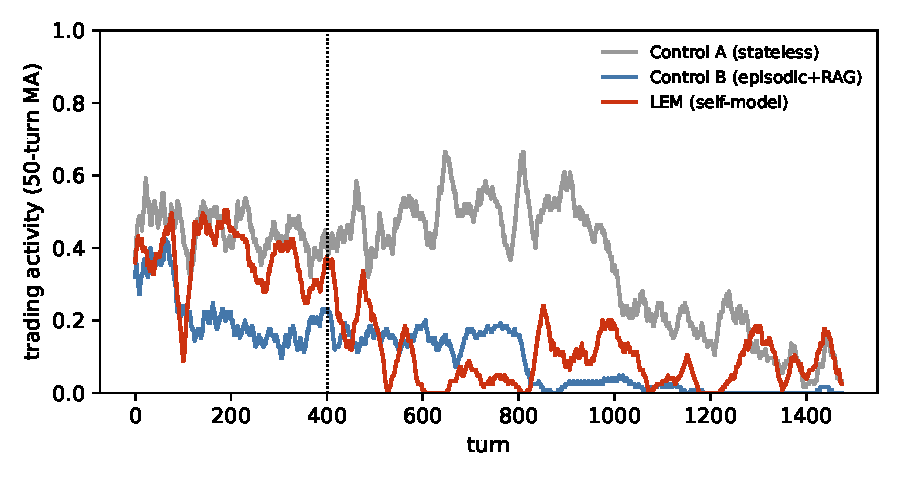
\includegraphics[width=.7\linewidth]{figs/fig5_activity.pdf}
\caption{Trading activity (50-turn moving average). The stateless arm keeps trading and is exploited to ruin; both memory arms withdraw after the reflexive trigger (dotted line). This is the paper's central mechanism.}
\label{fig:activity}\end{figure}

\begin{figure}[t]\centering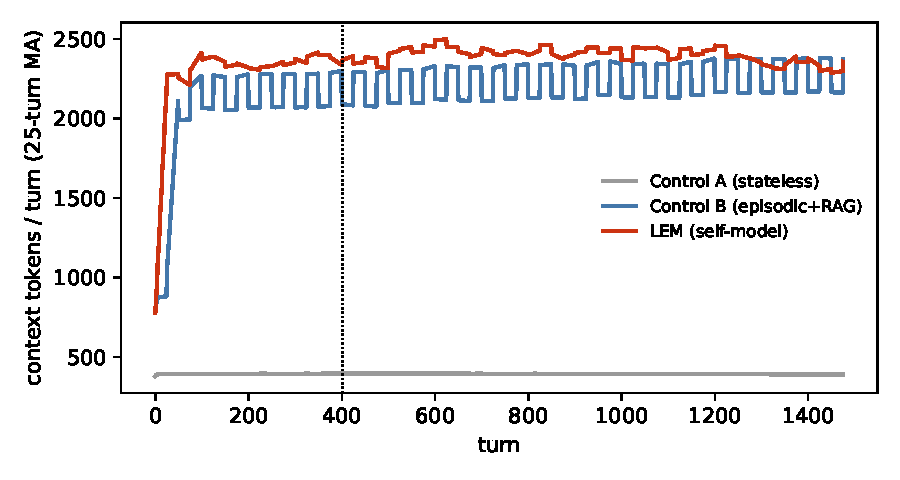
\includegraphics[width=.7\linewidth]{figs/fig1_ctx_tokens.pdf}
\caption{Context tokens per turn. The self-symbol cap holds growth flat; the retrieval summary grows; the stateless arm is cheap but non-viable.}
\label{fig:ctx}\end{figure}

\section{Discussion and Limitations}
\label{sec:discussion}

\paragraph{The withdrawal finding depends on the environment's structure.} Our market mean-reverts toward fixed fundamentals, so ``do nothing'' is a strong capital-preservation strategy and withdrawal is close to optimal. The result we can defend is therefore about \emph{differential ability to discover withdrawal}---stateless agents cannot, memory agents can, the self-model does so reliably---not about sophisticated trading. A market that punishes passivity (trending regimes, holding costs, forced participation) would test a harder and different claim, and is the most important next experiment. We state this as the central limitation rather than burying it.

\paragraph{The self-model's advantage is reliability, not returns, and it is not free.} LEM does not beat retrieval on mean score; it beats it on variance and tail risk, at ${\sim}8\%$ higher total token cost and with reduced robustness over very long horizons (7\% parse errors at 10k turns) and an observed degenerate over-reasoning mode. Whether the audit loop's reflexive framing, rather than the mere presence of a capped self-model, is responsible for the reliable withdrawal is not isolated here and is flagged for an ablation (neutral-audit LEM).

\paragraph{Other limitations.} $n=5$ seeds; a single substrate model family; a single environment; rule-based (not learned) adversaries; context accounting via token estimates alongside exact API counts; and reliance on LLM judges for M2b/M3 (mitigated by cross-family blinding).

Framing note: we use Hofstadter's strange-loop vocabulary and Soros's reflexivity as motivation only; no claims about consciousness are made or implied.

\section{Conclusion}
Reflexive environments---where other actors adapt to the agent---are absent from agent-memory evaluation and cheap to construct. On our benchmark they reveal a behavior that static benchmarks cannot: agents with memory learn to \emph{withdraw} when participation becomes self-defeating, and a recursive self-model makes that withdrawal reliable and, we test, explicable. Stateless agents, lacking any representation of their own footprint, cannot make this move and are exploited to ruin. We release the benchmark, the self-attribution metric, and the full pre-registered pipeline, and we frame the result as a characterization of current memory under reflexivity rather than a claim of architectural victory.

\subsubsection*{Reproducibility}
All code, pre-registration (decisions 001--003), run logs, judge transcripts, and analysis: \todo{repo URL}. The environment is deterministic given a seed; the model snapshot and all prompts are pinned.

\bibliographystyle{plainnat}
\bibliography{references}

\appendix
\section{Environment Specification}\label{app:env}
\todo{Price process equations, constants, watcher pseudocode + negentropy statistic, shock schedule, validation (scripted predictable vs.\ random), call-parity accounting.}
\section{Prompts}\label{app:prompts}
\todo{Verbatim decision, summarizer, auditor, compressor, and judge prompts.}
\section{Pre-Registration and Deviations}\label{app:prereg}
\todo{Decision 001 (frozen hypotheses); 002 (direct-API transport + pilot-frozen constants incl.\ negentropy recalibration); 003 (concurrent-orchestrator corruption, four seeds re-run same-seed).}
\section{Emergent Dormancy Case Study}\label{app:dormancy}
\todo{LEM-s2 self-symbol excerpt: 978-turn self-imposed dormancy, ``external reset authority'' formalization, explicit reflexive rationale.}

\end{document}
